\chapter{REVISÃO DA LITERATURA}
\label{cap:revisao}

Este capítulo tem como objetivo apresentar os principais conceitos à respeito do sistema proposto, além de indicar um estudo sobre o estado da arte do sistema proposto.

\section{Veículos Inteligentes e Automação Veicular}

A revolução tecnológica que diversos setores têm experimentado se aplica também ao ramo automobilístico. Desde que o primeiro veículo automotor ganhou as ruas no século XIX, tecnologias vem sendo empregadas de forma contínua de tal forma a proporcionar conforto, segurança e economia aos usuários de veículos. Atualmente, a maioria dos veículos em circulação possuem algumas destas tecnologias, como os freios ABS (\textit{Anti-Lock Braking System}) e Programas de Estabilidade Eletrônica (ESP: \textit{Electronic Stability Program}), que de forma contundente proporcionam segurança aos condutores e passageiros por meio do uso de sistemas eletrônicos de alta qualidade.

Esta evolução tecnológica se deve muito à popularização de dispositivos semicondutores que deu início à Era dos Computadores na década de 1970, onde, visto o que o uso de sistemas microprocessados poderiam proporcionar, já se começou a imaginar um futuro onde veículos completamente autônomos estariam inseridos no mercado. A Figura~\ref{fig:aut_car60} apresenta o conceito de veículo autônomo imaginado nos anos de 1960, onde se idealiza um veículo seguidor de linha, sem a necessidade de condutores.

\begin{figure}[!htb]
\centering
\caption{Conceito de carro autônomo na década de 1960.} %legenda
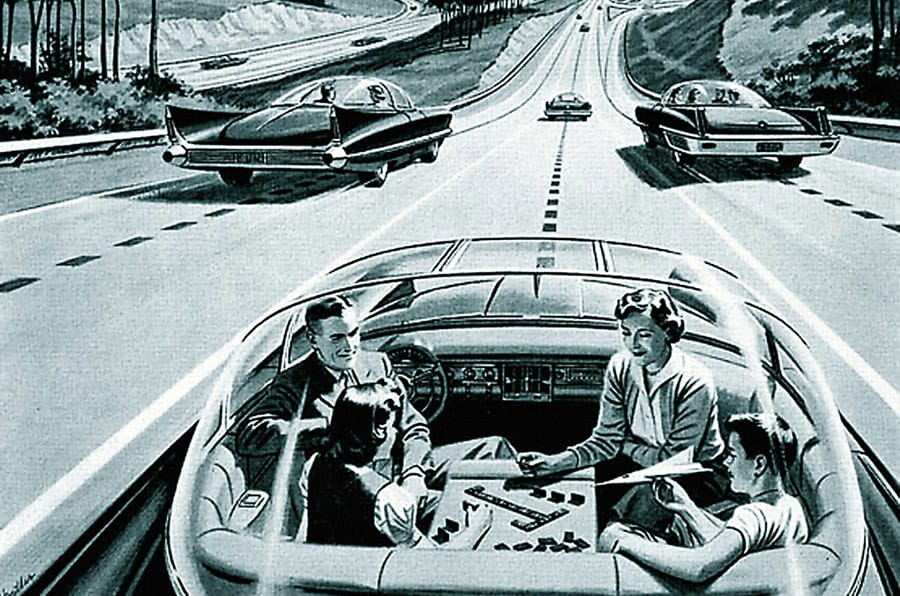
\includegraphics[scale=0.4]{aut_car.jpg}\\  % o 0.9 indica 90% do tamanho original
% pdfLaTeX aceita figuras no formato PNG, JPG ou PDF
% figuras vetoriais podem ser exportadas para eps e depois convertidas para pdf usando epstopdf
{\small Fonte: Auto-Medienportal.Net/Wikipedia} %Fonte da imagem
\label{fig:aut_car60} %rotulo para refencia
\end{figure}

Seguindo a evolução e popularização dos microprocessadores, surgiram assim as Unidades de Controle Eletrônico (ECU). Na indústria automotiva, uma ECU é um dispositivo eletrônico embarcado que realiza a leitura de sinais oriundos de sensores localizados em diversas partes e componentes do veículo e dependendo destas informações colhidas controla várias partes importantes do veículo, como o motor e outras opções automatizadas do veículo \cite{Ebert2009}.

A grande quantidade de informações que passou a circular entre ECU's fez com que surgisse a necessidade de desenvolver uma rede de comunicação multiplexada entre as ECU's, de tal forma a simplificar o cabeamento e reduzir custos de implementação. Assim na década de 80, foi desenvolvido pela Bosch a \textit{Controller Area Network}, ou CAN-bus, que é um barramento intraveicular de comunicação entre ECU's, sensores e atuadores. O CAN-bus é conhecido por sua robustez na transmissão de dados, sendo resistente à interferências eletromagnéticas, e operação em tempo real \cite{Tuohy2014b}. Sendo assim, a crescente capacidade de processamento das ECU's, aliado à grande quantidade de informações relevantes disponíveis no CAN-bus, proporcionaram a introdução do conceito de veículos inteligentes.

Veículos inteligentes, segundo \citeonline{Hubaux2004}, são veículos que são capazes de perceber o ambiente no qual estão inseridos. Um veiculo inteligente deve estar equipado com registradores de dados, processadores, sistemas de posicionamento e geolocalização,  sensores que permitam que o veículo esteja "ciente" do ambiente, seja no contexto intraveicular, ou no contexto extraveicular. 

No contexto intraveicular, o veículo está ciente de diversos fatores no que diz respeito ao comportamento do condutor, tais como a percepção de fatores neurofisiológicos que podem comprometer a segurança dos usuários, como detecção de sonolência, agressividade ou embriaguez, através de padrões de direção característicos de cada situação. 

No que diz respeito ao contexto extraveicular, o veículo percebe uma série de situações que podem comprometer a segurança dos usuários e, consequentemente, alertar ou até mesmo intervir na dinâmica de direção de modo evitar qualquer casualidade. Como exemplos pode-se citar o monitoramento de pontos cegos do veículo, como uma forma de proporcionar ultrapassagens seguras. Sistemas de estacionamento automatizado são outro exemplo deste tipo de sistema, onde o veículo monitora os objetos que o rodeiam e realiza a manobra de estacionamento de forma automática. Outro sistema que visa garantir a segurança dos usuários é o controle de velocidade de cruzeiro, onde o veículo realiza o ajuste da velocidade de acordo com a distância entre o veículo hospedeiro e os veículos à frente. Este sistema é baseado na velocidade do veículo à frente o veículo hospedeiro desacelera ou acelera até a velocidade limiar, tal que a distância entre os veículos seja a estipulada para a segurança dos usuários.

A medida que os veículos inteligentes passam a ser mais sensitivos ao ambiente, mais próximos à total automatização da direção eles estão. Segundo \citeonline{DeWinter2014}, diversos grupos de pesquisa em todo o mundo focam no estudo de veículos autônomos com o objetivo de uma inserção revolucionária do produto no mercado, porém, na prática este processo é mais evolucionário que revolucionário. Isto se dá pelo fato que ano após ano, novas tecnologias de assistência ao condutor (assunto a ser tratado na próxima seção) são inseridos no mercado, e assim mais automatizada se torna a direção. 


Segundo a norma J3016 da \citeonline{sae2014}, existem seis níveis de automação veicular, desde não automatizado até totalmente automatizado. Dos níveis 0 ao 2 é esperado que o \textit{Condutor Humano} monitore o ambiente de direção e que seja responsável pelas decisões tomadas, porém podem existir sistemas que auxiliem o condutor na tomada de decisões. Por sua vez, nos níveis de 3 a 5, o responsável pelo monitoramento de direção é o \textit{Sistema de Direção Automático}, que pode ser definido como a combinação de diversos sistemas de assistência ao condutor (DAS), porém dos quais não estão inclusos sistemas de intervenção e advertência momentânea pelo fato de não automatizarem partes da tarefa dinâmica de direção e, consequentemente, não mudarem o papel do condutor humano. Os seis níveis de automatização da direção são:

\begin{itemize}
	\item \textbf{SAE Nível 0 - Não Automatizado:} O condutor humano controla todos os aspectos da tarefa dinâmica de condução, mesmo quando auxiliado por sistemas de alerta e intervenção. O condutor humano é responsável pelo monitoramento do ambiente.
	
	\item \textbf{SAE Nível 1 - Assistência ao Condutor:} O modo de direção-execução específica é feito pelo sistema ou pelo condutor, tanto na direção, quanto na aceleração/desaceleração, usando informações do ambiente  enquanto o condutor humano é responsável por todas os outros aspectos da dinâmica de condução.
	
	\item \textbf{SAE Nível 2 - Automação Parcial:} O modo de direção-execução específica é feito por um ou mais sistemas de assistência, tanto na direção, quanto na aceleração/desaceleração, usando informações do  ambiente enquanto o condutor humano é responsável por todas os outros aspectos da dinâmica de condução.
	
	\item \textbf{SAE Nível 3 - Automação Condicional:} O modo de direção específica é feito por um sistema automatizado de condução  em todos os aspectos da tarefa dinâmica de condução com a expectativa de que o condutor humano assuma o controle se requisitado.
	
	\item \textbf{SAE Nível 4 - Altamente Automatizado:} O modo de direção específica é feito por um sistema  automatizado de condução em todos os aspectos da tarefa dinâmica de condução, mesmo que o condutor humano não assuma o controle apropriadamente quando requisitado.
	
	\item \textbf{SAE Nível 5 - Totalmente Automatizado:} O modo de direção específica é feito por um sistema  automatizado de condução em todos os aspectos da tarefa dinâmica de condução sob quaisquer condições ambientais.

\end{itemize}

Como exemplificação destes níveis de automatização, a Figura~\ref{fig:adas2ad} ilustra os tipos de tecnologias em cada nível SAE, desde somente sistemas avançados de assistência ao condutor, até sistemas de direção automatizados.


\begin{figure}[!htb]
\centering
\caption{Exemplos de sistemas de automatização em diferentes níveis.} %legenda
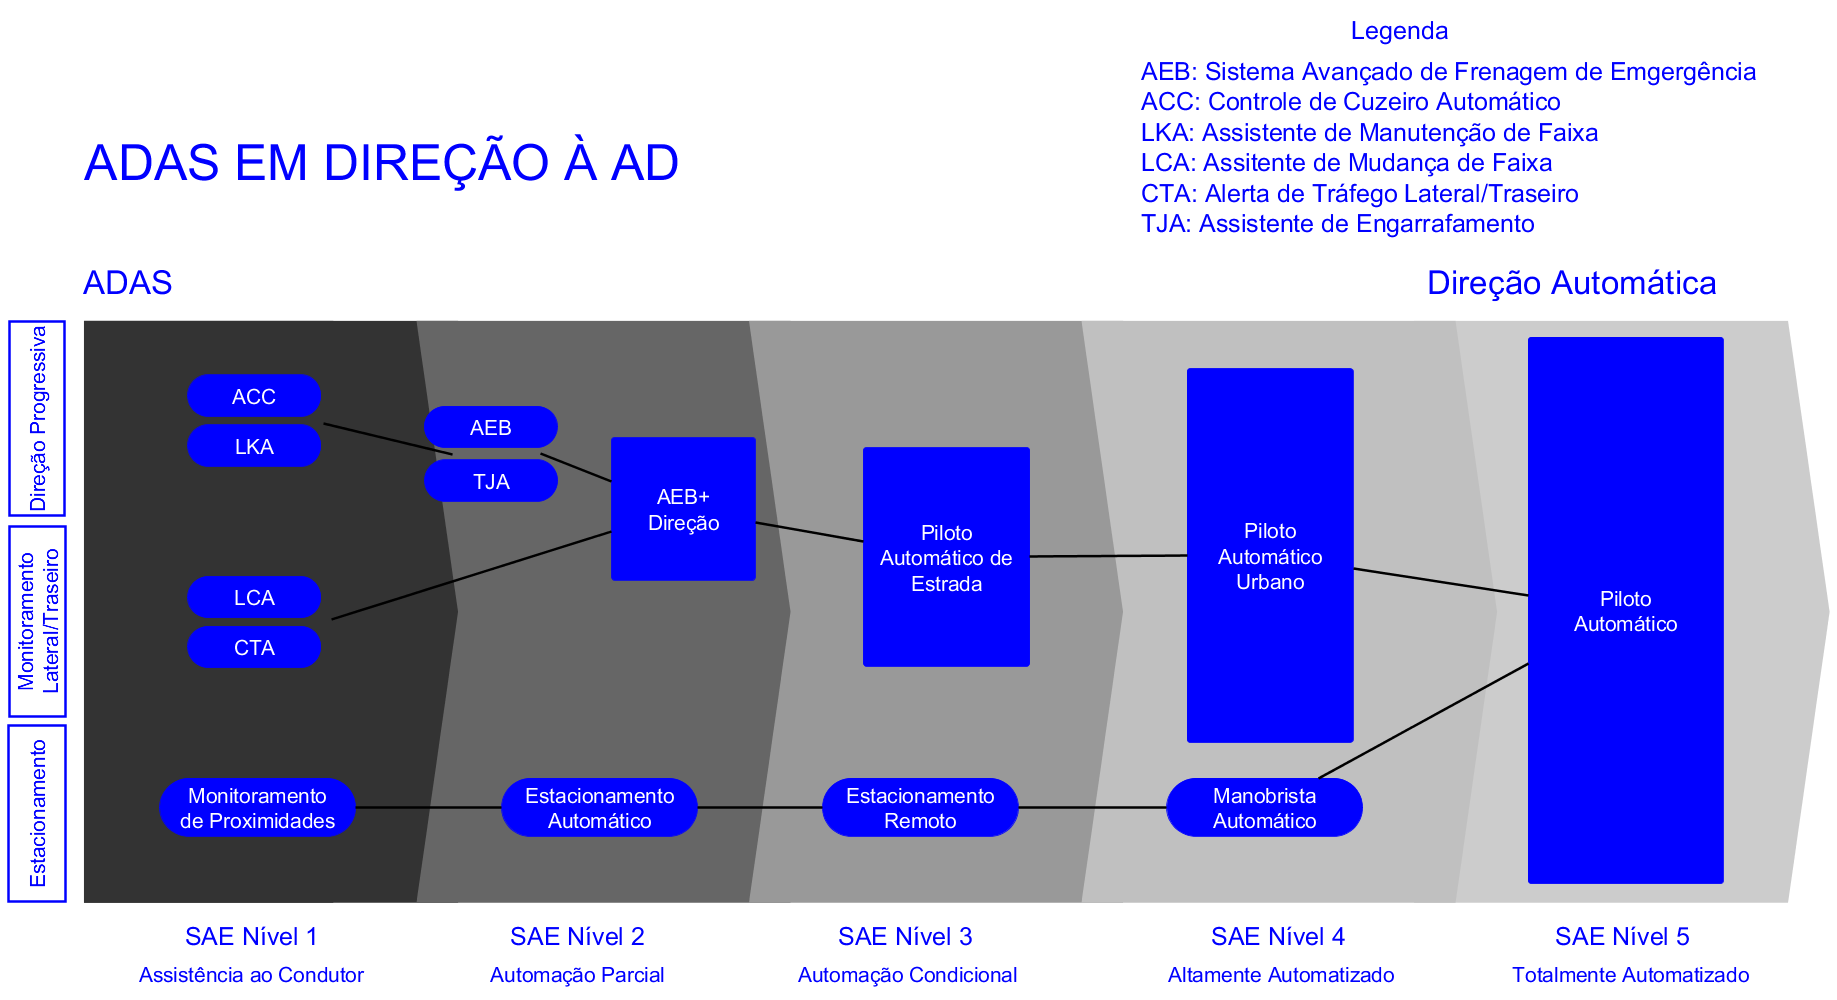
\includegraphics[scale=0.27]{adas2ad.png}\\  % o 0.9 indica 90% do tamanho original
% pdfLaTeX aceita figuras no formato PNG, JPG ou PDF
% figuras vetoriais podem ser exportadas para eps e depois convertidas para pdf usando epstopdf
{\small Fonte: Adaptado de \citeonline{Renesas2017}} %Fonte da imagem
\label{fig:adas2ad} %rotulo para refencia
\end{figure}



\section{Sistemas Avançados de Assistência ao Condutor (ADAS)}

%Desde que o primeiro veículo automotor à combustão interna foi concebido por Carl Benz em 1886, a indústria  automobilística tem experimentado uma constante expansão e penetração em diferentes mercados. Isso se reflete no fato de que a qualidade de vida de uma determinada população é correlacionada com a sua capacidade de mobilidade. Contudo, esta expansão trás à tona uma série de desafios. Além de, obviamente, da redução dos custos financeiros da produção, o consumo de combustível e a implementação e manutenção da infraestrutura (estradas, entre outros) passa por custos de ordem econômico, ambiental e social. Sendo assim a evolução e expansão passa pela redução do consumo de recursos naturais, emissão de gases de efeito estufa e poluição sonora. Somado a isso, fomenta-se a preocupação com congestionamento crescente experimentado por centros urbanos e acidentes de trânsito, umas das principais causa de óbitos e feridos ao redor do mundo.
%
%Hoje, o foco da indústria automotiva pode ser dividido em duas frentes. Em países em desenvolvimento, a indústria tem como foco a redução de custos da produção de tal modo que a oferta de seus produtos se estenda para a população com menor poder aquisitivo. No Brasil, por exemplo, fabricantes têm apostado em carros compactos com baixo consumo de combustível e custo de produção reduzido. Como o pioneiro em sua categoria o Volkswagen Up!, introduzido em 2011, seguido pelo Fiat Mobi (2016) e o Renault Kwid (2017). Porém, tais veículos mencionados são considerados básicos em termos tecnológicos, uma vez que não dispõem de tantos recursos de segurança e conforto aos usuários, com objetivo de justamente oferecer um produto acessível.
%
%Por sua vez, países desenvolvidos, como a Alemanha e Reino Unido, já possuem uma grande penetração de mercado, ou seja, a oferta de veículos à população já está consolidado e quase saturado. Esta situação faz com que as fabricantes de automóveis objetivem a qualidade de seus produtos e a experiência dos usuários. Dentre tais objetivos estão tecnologias que previnam casualidades, reduzam o impacto ambiental e, como consequência, se aumente a eficiência móvel em termos de energia, tempo e recursos.
%
%Um termo frequentemente discutido é a eletrificação dos automóveis que visam reduzir o custo ambiental e conter a crescente escassez de recursos.
%
%
%Contudo, essa expansão trouxe à tona uma série de problemas 

Acidentes de trânsito são uma das maiores causas de mortes na atualidade. A maioria dos acidentes de trânsito são provocados pela desatenção e imprudência dos condutores. Segundo \citeonline{Hoess2009}, 97\% são causados por falha humana. Contudo grande parte dos estudos são voltados para macro-problemas, como o número de veículos nas vias e gerenciamento de tráfego, e não dão atenção suficiente para decisões individuais de condutores e como isso impacta no tráfego \cite{Carmona2015}. 
Portanto, assistência ao condutor em diferentes níveis são ferramentas potenciais para a segurança dos usuários de veículos e pedestres. Ciente disso, os recentes avanços em inteligência computacional e técnicas de percepção têm proporcionado uma série de novas aplicações desenvolvidas com o propósito de prevenir estes tipos de casualidades utilizando o conceito chamado de Sistemas Avançados de Assistência ao Condutor, ou simplesmente ADAS (\textit{Advanced Driver Assistace System}). 

Segundo \citeonline{Saito2016} os ADAS são baseados em modelos de automação e  podem ser categorizados em quatro classes:

\begin{enumerate}
	\item Percepção Aumentada: São todos os sistemas que têm por finalidade monitorar situações em que normalmente o condutor não tem condições de controlar com precisão. Como exemplo estão sensores de estacionamento, monitoramento de ponto cego em mudança de faixa ou ultrapassagem. 
	
	\item Aleta para riscos potenciais: Sistemas que têm intuito de advertir o condutor sobre alguma situação de risco, tais como sonolência/fadiga, pouca distância ao veículo à frente, alerta sobre sobre possíveis falhas nos sistemas do veículo se enquadram nesta classe.
	
	\item Avisos desencadeados: São sistemas que solicitam ao condutor que tome uma ação específica em uma determinada situação de risco. Como exemplos estão alertas de velocidade alta e detecção de sonolência.
	
	\item Controle de segurança automático: Este sistema é acionado quando o condutor não toma providências quando alertado ou a ação de controle do condutor é insuficiente para tal situação de risco.
	
\end{enumerate}

As classes 1 e 2 são implementadas para auxiliar o condutor a perceber ou entender o contexto. Este entendimento/percepção determina quais ações devem ser tomadas. Uma vez que decisão de diagnóstico de situação é feita, a seleção de ações geralmente é a adequada. Contudo, a decisão tomada pelo condutor pode não ser a correta. Assim a classe 3 auxilia o condutor em tal circunstância. Qualquer ADAS que utiliza as classes 1, 2 e 3 são compatíveis com o princípio de automação centrada no ser humano, onde o condutor humano é a autoridade final no processo de automação. Se o ADAS conter a classe 4, a autoridade passa a ser dividida entre o sistema e o humano. Existem controvérsias sobre o uso da classe 4, uma vez que máquinas altamente automatizadas podem trazer efeitos negativos, como falhas em sensores, erros na malha de controle, complacência, excesso de confiança no sistema, entre outros \cite{Inagaki2012}.


%\section{Modelagem e Identificação de Comportamento do Condutor}

\section{Inteligência Computacional Aplicado à Identificação de Comportamento do Condutor}


A revisão bibliográfica feita por \citeonline{Meiring2015} aborda quais algoritmos de inteligência artificial são mais adequados para análise de estilos de direção e comportamento de condutores. É abordado quais os tipos de direção, bem como as causas e consequências de cada um deles (normal/seguro, agressivo, desatento (fadiga, distração), alcoolizado), e aponta o potencial de tais algoritmos em detectar tais condições e prevenir casualidades proporcionadas pelas mesmas. É também realizada uma classificação de técnicas de inteligência computacional e suas aplicações mais comuns são apresentadas na Tabela \ref{tecs1}. Técnicas de inteligência computacional e suas aplicações em ADAS. É concluído que os algoritmos mais promissores para criação de aplicações futuras em ADAS são técnicas baseadas em Lógica Fuzzy, implementação de Modelos Ocultos de Markov (HMM) e Máquinas de Vetor de Suporte (SVM).

\begin{table}[!htb]
	\centering
	\caption{Técnicas de inteligência computacional e suas aplicações em ADAS. }
	\label{tecs1}
	\begin{tabular}{p{55mm}|p{95mm}}
		\hline
		\multicolumn{1}{c|}{\textbf{Técnica}} & \multicolumn{1}{|c}{\textbf{Aplicações}}                                                                                            \\ \hline
		Redes Neurais Artificiais              & Detecção de sonolência e distração, predição do comportamento do volante, visão computacioal.                                       \\ \hline
		Fast Fourier Transform                 & Detecção de sonolência.                                                                                                             \\ \hline
		Clusterização                          & Distinção de estilo de direção e rotulação de condutor.                                                                             \\ \hline
		Clusterização K-means                  & Identificação individual de condutor e monitoramento de condições de rota.                                                          \\ \hline
		Máquina de estados                     & Reconhecimento de manobras.                                                                                                         \\ \hline
		Máquina de estados finitos             & Modelagem de tomadas de decisão do condutor.                                                                                        \\ \hline
		Máquina de estados híbridos            & Veículos Autônomos.                                                                                                                 \\ \hline
		Lógica Fuzzy                           & Detecção de fadiga, identificação de distração, métodos de pontuação e métodos de reconhecimento de estilo de direção.              \\ \hline
		Modelos Ocultos de Markov (HMM)        & Estimação de comportamento do condutor, reconhecimento de manobras, análise de performance de direção e identificação de distração. \\ \hline
		Técnicas Bayesianas                    & Estimação de comportamento do condutor em situações de dados faltantes.                                                             \\ \hline
		Árvores de decisão                     & Estimação de confiança de resultados em fusão de dados para detecção de sonolência.                                                 \\ \hline
		Modelo de misturas de gaussianas       & Identificação de distração, reconhecimento de manobras e monitoramento de condições de rota.                                       \\ \hline
		Dynamic time warping (DTW)             & Classificação de perfil de risco do condutor e assistentes de direção ou alerta de segurança.                                       \\ \hline
		Filtros de Kalman                      & Predição de processos e modelagem de comportamento humano.                                                                          \\ \hline
		Máquinas de vetor de suporte (SVM)     & Métodos de reconhecimento de estilo de direção, detecção de sonolência e estimação de estado do veículo.                            \\ \hline
		Algoritmos Genéticos                   & Calibração de processos de modelagem de carros adjacentes.                                                                          \\ \hline
	\end{tabular}
\centering {\small Fonte: Adaptado de \citeonline{Meiring2015}.} %Fonte do quadro
\end{table}

Em seu trabalho, \citeonline{Kumtepe2016} propõem um modelo que faz a fusão de dados provenientes de sensores disponíveis no carro e por meio de câmeras com o objetivo de se decidir se o condutor apresenta sinais de agressividade ou desatenção. Estas informações são usadas para formar o vetor de características que representam o comportamento do condutor e então são submetidos à uma máquina de vetores de suporte (SVM) a fim de se classificar o condutor testado. O método proposto obteve uma taxa de detecção de agressividade por parte do condutor de 93.1\%.

Por sua vez, \citeonline{Blaszczyk2014} realiza experimentos controlado, onde dois condutores são submetidos a um teste em circuito fechado e dados são coletados por meio da interface OBD-II e Raspberry Pi, além do uso de sensores embarcados em um \textit{smartphone}, com o objetivo de diferencia-los. Utilizando quatro técnicas de classificação (Processo Gaussiano, M5P, \textit{M5Rules} e Tabela de Decisões). O erro médio quadrático (RMSE) para Processo Gaussiano, M5P, \textit{M5Rules} e Tabela de Decisões, foi, respectivamente 0.168, 0.087, 0.023 e 0. Apesar do erro relativamente baixo, é importante ressaltar que somente dois condutores foram comparado, necessitando assim de mais testes a fim de comprovar a eficácia do sistema.

Seguindo outra vertente, \citeonline{Castignani2015} faz uso somente de \textit{smartphones} para monitorar o comportamento do condutor e alertar para possíveis situações de risco. O uso do dispositivo se justifica pela sua atual penetração no mercado e a facilidade de desenvolvimento de aplicativos, além da robustez dos sensores embarcados nos aparelhos. Um sistema fuzzy é usado para computar o escore de diferentes condutores usando informações em tempo real, como acelerômetros e sistema de navegação GPS provenientes do \textit{smartphone}, aceleração, frenagens e posição do volante, provenientes do barramento CAN do veículo por meio da interface OBD-II, além de topologia da rota e condições climáticas. A validação do sistema é feita por meio de teste em circuito fechado com diversos condutores.

Técnicas de inteligência computacional híbridas também são exploradas, como no trabalho de \citeonline{Echanobe2016}, onde uma Rede Neural Artificial (RNA) é otimizado por meio de Algorítimos Genéticos Multiobjetivos com a finalidade de realizar a classificação de condutores por meio de diversos parâmetros de entrada. Testes foram conduzidos com diferentes parâmetros e número de neurônios e camadas, a fim de diminuir o erro da RNA. O resultado obtido é um um classificador com menor número de variáveis de entrada em diferentes domínios (tempo, frequência e cepstral), menor número de neurônios e camadas escondidas da RNA e por consequência um sistema mais rápido eficiente no que diz respeito ao custo computacional.

Contudo, \citeonline{Piotr2015} afirma que a modelagem de comportamento de condutor ainda não são confiáveis o suficiente para aplicação em larga escala, justificando que grande parte dos trabalhos na área foram feitos com experimentos limitados pela quantidade de condutores testados e que somente os sensores utilizados não são suficientes para tal modelagem. Isto ocorre uma vez que as decisões tomadas não são repetitivas, tal qual assumindo por diversos trabalhos. Em cenários repetitivos é possível distinguir entre diferentes tipos de comportamentos, porém, quando o mesmo condutor é submetido a cenários diferentes, a correlação entre os dados é reduzida e muitas vezes é comparada com outro condutor. 

